\documentclass[11pt, oneside]{article}   	% use "amsart" instead of "article" for AMSLaTeX format
\usepackage{geometry}                		% See geometry.pdf to learn the layout options. There are lots.
\geometry{letterpaper}                   		% ... or a4paper or a5paper or ... 
%\geometry{landscape}                		% Activate for for rotated page geometry
%\usepackage[parfill]{parskip}    		% Activate to begin paragraphs with an empty line rather than an indent
\usepackage{graphicx}				% Use pdf, png, jpg, or eps� with pdflatex; use eps in DVI mode
								% TeX will automatically convert eps --> pdf in pdflatex		
\usepackage{amssymb}
\usepackage{amsmath}
\usepackage{parskip}
\usepackage{color}

\title{Newton to Kepler}
%\author{The Author}
%\section{}
% \subsection*{R code}
\date{}							% Activate to display a given date or no date

\graphicspath{{/Users/telliott_admin/Dropbox/Tex/png/}}

% \begin{center} 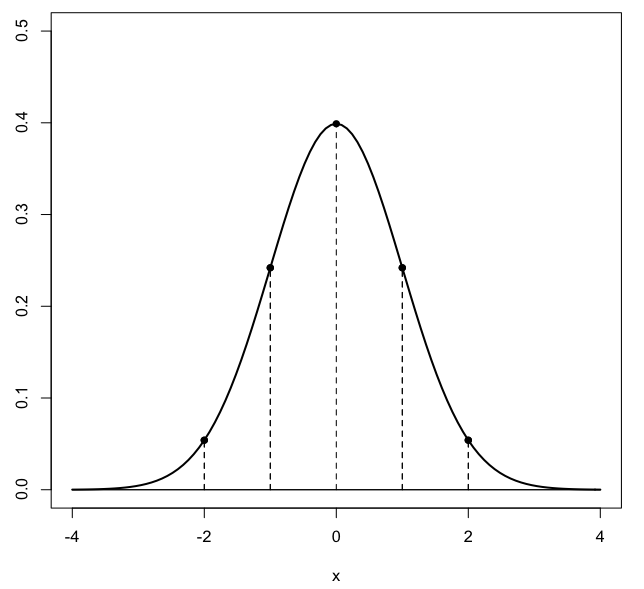
\includegraphics [scale=0.4] {gauss3.png} \end{center}

\begin{document}
\maketitle
\Large
\noindent

The last part of Varberg's derivation is about K3.  To prove:
\[ T^2 = \frac{(2 \pi)^2}{GM} \ a^3 \]
where $T$ is the period, $GM$ is our constant from before, and $a$ is the length of the half-major axis of the ellipse.  In other words, the period of an orbit is the $3/2$ power of the "radius", technically the semi-major axis of the ellipse.

Start with K2
\[ 2 \ \frac{dA}{dt} =  h \]
Integrate with respect to time over one revolution obtaining an ellipse with area $\pi a b$ and the period $T$ for the time
\[ 2 \pi a b = hT \]
\[ T^2 = (\frac{2 \pi a b}{h})^2 \]
Now, go back to the equation for the orbit
\[ r(1 + e \cos \theta) = \frac{h^2}{GM} \]
Consider one-half an orbit between $\theta = 0 \rightarrow \theta = \pi$.  The length of the axis is $2a$, equal to $2r$ for this orbit, so
\[ 2a = \frac{h^2}{GM(1 + e \cos \pi)} +  \frac{h^2}{GM(1 + e \cos 0)} \]
\[ = \frac{h^2}{GM} (\frac{1}{1 - e} +  \frac{1}{1 + e}) \]
\[ = \frac{h^2}{GM} \ \frac{2}{1 - e^2} \]
So
\[ a = \frac{h^2}{GM} \ \frac{1}{1 - e^2} \]
For an ellipse
\[ \frac{b^2}{a^2} = 1 - e^2 \]
so
\[ a = \frac{h^2}{GM} \ \frac{a^2}{b^2} \]

\[  b^2 = \frac{ah^2}{GM}  \]
We had 
\[ T^2 = (\frac{2 \pi a b}{h})^2 \]
\[ = (\frac{2 \pi a }{h})^2 \  \frac{ah^2}{GM}  \]
\[ = \frac{(2 \pi)^2}{GM} a^3 \]
which is K3.  $GM$ is the gravitational constant times the mass of the sun.  The term due to the angular momentum $h$ has dropped out.

Note that we can get an estimate for $GM$ from observation of the orbits of the planets, and that $G$ can be determined very simply, allowing us to find $M$, and "weigh the sun".

\end{document}  